% =====================================================================
%  Introduction to Neuroscience — Session 9: Activity booklet (The spike)
%  Companion to NEUR_S09_action_potential. Page numbers are referred to on
%  the slides; keep the \newpage breaks. Spike Lab link: \lablink below.
% =====================================================================
\documentclass[12pt,a4paper]{article}
\usepackage[margin=1.9cm,bottom=2.2cm]{geometry}
\usepackage[T1]{fontenc}
\usepackage{helvet}
\renewcommand{\familydefault}{\sfdefault}
\usepackage{setspace}
\setstretch{1.18}
\usepackage{ragged2e}
\usepackage{enumitem}
\usepackage{array}
\usepackage{booktabs}
\usepackage{xcolor}
\usepackage{amssymb}
\usepackage{tikz}
\usetikzlibrary{arrows.meta}
\usepackage{tcolorbox}
\tcbuselibrary{skins}
\usepackage{fancyhdr}
\usepackage{textcomp}
\usepackage{pgfplots}
\pgfplotsset{compat=1.17}
\usepackage{qrcode}
\usepackage{url}
\urlstyle{sf}

\newcommand{\sessnum}{9}  % change here if the session is renumbered
\definecolor{kprimary}{HTML}{1F3A5F}
\definecolor{kaccent}{HTML}{B85A0E}
\definecolor{kgreen}{HTML}{23665A}
\definecolor{kred}{HTML}{A12F24}
\definecolor{kpale}{HTML}{F7F3EA}
\definecolor{kgrey}{HTML}{4B5563}

\pagestyle{fancy}\fancyhf{}
\renewcommand{\headrulewidth}{0pt}
\fancyfoot[L]{\small\color{kgrey}Introduction to Neuroscience \,$\cdot$\, Session \sessnum\ activity booklet}
\fancyfoot[R]{\small\bfseries\color{kprimary}Page \thepage}
\setlength{\parindent}{0pt}
\setlength{\parskip}{4pt}
\hyphenpenalty=10000 \exhyphenpenalty=10000 \tolerance=9000 \emergencystretch=3em
\RaggedRight
\setlist{itemsep=3pt,topsep=4pt}

\newcommand{\pagehead}[1]{{\color{kprimary}\LARGE\bfseries #1}\par\vspace{2pt}{\color{kaccent}\rule{\linewidth}{1.2pt}}\par\vspace{4pt}}
\newcommand{\infopill}[2]{{\setlength{\fboxsep}{4pt}\fcolorbox{kaccent}{kaccent!8}{\textbf{#1:}\ #2}}}
\newcommand{\actinfo}[3]{\infopill{Time}{#1}\hspace{0.5em}\infopill{Who}{#2}\hspace{0.5em}\infopill{You need}{#3}\par\medskip}
\newcommand{\lines}[1]{\par\foreach \i in {1,...,#1}{\vspace{0.75cm}\hrule height 0.4pt}\par\medskip}
\newcommand{\blank}[1][3.2cm]{\rule{#1}{0.4pt}}
\newcommand{\cb}{$\square$\ }
\newtcolorbox{stepsbox}[1][]{enhanced,colback=kpale,colframe=kprimary,arc=2mm,boxrule=0.8pt,left=8pt,right=8pt,top=5pt,bottom=5pt,
  halign=flush left,title={\bfseries Steps (tick each one when done)},fonttitle=\normalsize,coltitle=white,#1}
\newtcolorbox{infobox}[1][]{enhanced,colback=kprimary!4,colframe=kprimary!70,arc=2mm,boxrule=0.6pt,left=8pt,right=8pt,top=4pt,bottom=4pt,
  halign=flush left,fonttitle=\normalsize\bfseries,coltitle=white,#1}
\newtcolorbox{studycard}[1][]{enhanced,colback=white,colframe=kgreen,arc=2mm,boxrule=0.8pt,left=7pt,right=7pt,top=3pt,bottom=3pt,
  halign=flush left,fonttitle=\normalsize\bfseries,coltitle=white,#1}


% ---------- at-a-glance additions (v2), same as the deck ----------
\definecolor{cNa}{HTML}{B85A0E}
\definecolor{cK}{HTML}{6A3D9A}
\definecolor{cCl}{HTML}{23665A}
\definecolor{cCa}{HTML}{A12F24}
\newcommand{\Na}{\textcolor{cNa}{\textbf{Na$^{+}$}}}
\newcommand{\K}{\textcolor{cK}{\textbf{K$^{+}$}}}
\tikzset{
  ionNa/.style={circle,fill=cNa,text=white,font=\footnotesize\bfseries,inner sep=0pt,minimum size=0.62cm},
  ionK/.style={circle,fill=cK,text=white,font=\footnotesize\bfseries,inner sep=0pt,minimum size=0.62cm},
  nb/.style={circle,fill=kprimary,text=white,font=\small\bfseries,inner sep=0pt,minimum size=0.55cm}}

\tikzset{badge/.style={circle,fill=kprimary,text=white,font=\scriptsize\bfseries,inner sep=0pt,minimum size=0.42cm}}
% ---- traces from the Hodgkin-Huxley (1952) model, same as Spike Lab ----
\newcommand{\apV}{(0.00,-65.00) (0.10,-65.00) (0.20,-65.00) (0.30,-65.00) (0.40,-65.00) (0.50,-65.00) (0.60,-65.00) (0.70,-65.00) (0.80,-65.00) (0.90,-65.00) (1.00,-65.00) (1.10,-65.00) (1.20,-65.00) (1.30,-65.00) (1.40,-65.00) (1.50,-65.00) (1.60,-65.00) (1.70,-64.99) (1.80,-64.99) (1.90,-64.99) (2.00,-64.87) (2.10,-63.63) (2.20,-62.45) (2.30,-61.32) (2.40,-60.22) (2.50,-59.12) (2.60,-58.01) (2.70,-56.84) (2.80,-55.57) (2.90,-54.15) (3.00,-52.61) (3.10,-51.79) (3.20,-50.43) (3.30,-48.36) (3.40,-45.22) (3.50,-40.21) (3.60,-31.48) (3.70,-14.97) (3.80,13.66) (3.90,36.81) (4.00,40.12) (4.10,38.05) (4.20,34.67) (4.30,30.52) (4.40,25.85) (4.50,20.86) (4.60,15.71) (4.70,10.52) (4.80,5.35) (4.90,0.28) (5.00,-4.68) (5.10,-9.51) (5.20,-14.22) (5.30,-18.80) (5.40,-23.31) (5.50,-27.77) (5.60,-32.27) (5.70,-36.94) (5.80,-41.96) (5.90,-47.57) (6.00,-53.96) (6.10,-60.96) (6.20,-67.56) (6.30,-72.27) (6.40,-74.70) (6.50,-75.70) (6.60,-76.05) (6.70,-76.17) (6.80,-76.19) (6.90,-76.17) (7.00,-76.14) (7.10,-76.11) (7.20,-76.07) (7.30,-76.02) (7.40,-75.98) (7.50,-75.93) (7.60,-75.88) (7.70,-75.83) (7.80,-75.78) (7.90,-75.72) (8.00,-75.67) (8.10,-75.61) (8.20,-75.55) (8.30,-75.49) (8.40,-75.42) (8.50,-75.36) (8.60,-75.29) (8.70,-75.22) (8.80,-75.15) (8.90,-75.08) (9.00,-75.00) (9.10,-74.93) (9.20,-74.85) (9.30,-74.77) (9.40,-74.69) (9.50,-74.60) (9.60,-74.52) (9.70,-74.43) (9.80,-74.34) (9.90,-74.25) (10.00,-74.16) (10.10,-74.06) (10.20,-73.97) (10.30,-73.87) (10.40,-73.77) (10.50,-73.67) (10.60,-73.57) (10.70,-73.47) (10.80,-73.37) (10.90,-73.26) (11.00,-73.15) (11.10,-73.05) (11.20,-72.94) (11.30,-72.83) (11.40,-72.72) (11.50,-72.61) (11.60,-72.50) (11.70,-72.39) (11.80,-72.27) (11.90,-72.16) (12.00,-72.05) (12.10,-71.93) (12.20,-71.82) (12.30,-71.70) (12.40,-71.59) (12.50,-71.47) (12.60,-71.36) (12.70,-71.24) (12.80,-71.13) (12.90,-71.01) (13.00,-70.90) (13.10,-70.78) (13.20,-70.67) (13.30,-70.55) (13.40,-70.44) (13.50,-70.32) (13.60,-70.21) (13.70,-70.10) (13.80,-69.99) (13.90,-69.88) (14.00,-69.77) (14.10,-69.66) (14.20,-69.55) (14.30,-69.44) (14.40,-69.33) (14.50,-69.22) (14.60,-69.12) (14.70,-69.01) (14.80,-68.91) (14.90,-68.81) (15.00,-68.70) (15.10,-68.60) (15.20,-68.50) (15.30,-68.40) (15.40,-68.31) (15.50,-68.21) (15.60,-68.11) (15.70,-68.02) (15.80,-67.93) (15.90,-67.83) (16.00,-67.74)}
\newcommand{\apNa}{(0.00,0.01) (0.10,0.01) (0.20,0.01) (0.30,0.01) (0.40,0.01) (0.50,0.01) (0.60,0.01) (0.70,0.01) (0.80,0.01) (0.90,0.01) (1.00,0.01) (1.10,0.01) (1.20,0.01) (1.30,0.01) (1.40,0.01) (1.50,0.01) (1.60,0.01) (1.70,0.01) (1.80,0.01) (1.90,0.01) (2.00,0.01) (2.10,0.01) (2.20,0.01) (2.30,0.02) (2.40,0.02) (2.50,0.03) (2.60,0.05) (2.70,0.06) (2.80,0.09) (2.90,0.12) (3.00,0.17) (3.10,0.23) (3.20,0.31) (3.30,0.42) (3.40,0.61) (3.50,0.98) (3.60,1.82) (3.70,4.15) (3.80,11.03) (3.90,23.16) (4.00,31.13) (4.10,32.98) (4.20,31.82) (4.30,29.56) (4.40,27.03) (4.50,24.53) (4.60,22.18) (4.70,19.99) (4.80,17.98) (4.90,16.13) (5.00,14.42) (5.10,12.85) (5.20,11.39) (5.30,10.04) (5.40,8.79) (5.50,7.60) (5.60,6.47) (5.70,5.37) (5.80,4.28) (5.90,3.17) (6.00,2.06) (6.10,1.08) (6.20,0.40) (6.30,0.10) (6.40,0.02) (6.50,0.00) (6.60,0.00) (6.70,0.00) (6.80,0.00) (6.90,0.00) (7.00,0.00) (7.10,0.00) (7.20,0.00) (7.30,0.00) (7.40,0.00) (7.50,0.00) (7.60,0.00) (7.70,0.00) (7.80,0.00) (7.90,0.00) (8.00,0.00) (8.10,0.00) (8.20,0.00) (8.30,0.00) (8.40,0.00) (8.50,0.00) (8.60,0.00) (8.70,0.00) (8.80,0.00) (8.90,0.00) (9.00,0.00) (9.10,0.00) (9.20,0.00) (9.30,0.00) (9.40,0.00) (9.50,0.00) (9.60,0.00) (9.70,0.00) (9.80,0.00) (9.90,0.00) (10.00,0.00) (10.10,0.00) (10.20,0.00) (10.30,0.00) (10.40,0.00) (10.50,0.00) (10.60,0.00) (10.70,0.00) (10.80,0.00) (10.90,0.00) (11.00,0.00) (11.10,0.00) (11.20,0.00) (11.30,0.00) (11.40,0.00) (11.50,0.00) (11.60,0.00) (11.70,0.00) (11.80,0.00) (11.90,0.00) (12.00,0.00) (12.10,0.00) (12.20,0.00) (12.30,0.00) (12.40,0.00) (12.50,0.00) (12.60,0.00) (12.70,0.00) (12.80,0.00) (12.90,0.00) (13.00,0.00) (13.10,0.00) (13.20,0.00) (13.30,0.00) (13.40,0.00) (13.50,0.00) (13.60,0.00) (13.70,0.00) (13.80,0.00) (13.90,0.00) (14.00,0.00) (14.10,0.00) (14.20,0.00) (14.30,0.00) (14.40,0.00) (14.50,0.00) (14.60,0.00) (14.70,0.00) (14.80,0.00) (14.90,0.00) (15.00,0.00) (15.10,0.00) (15.20,0.00) (15.30,0.00) (15.40,0.00) (15.50,0.00) (15.60,0.00) (15.70,0.00) (15.80,0.00) (15.90,0.00) (16.00,0.00)}
\newcommand{\apK}{(0.00,0.37) (0.10,0.37) (0.20,0.37) (0.30,0.37) (0.40,0.37) (0.50,0.37) (0.60,0.37) (0.70,0.37) (0.80,0.37) (0.90,0.37) (1.00,0.37) (1.10,0.37) (1.20,0.37) (1.30,0.37) (1.40,0.37) (1.50,0.37) (1.60,0.37) (1.70,0.37) (1.80,0.37) (1.90,0.37) (2.00,0.37) (2.10,0.37) (2.20,0.37) (2.30,0.37) (2.40,0.38) (2.50,0.39) (2.60,0.40) (2.70,0.41) (2.80,0.42) (2.90,0.44) (3.00,0.46) (3.10,0.48) (3.20,0.50) (3.30,0.53) (3.40,0.57) (3.50,0.62) (3.60,0.70) (3.70,0.83) (3.80,1.10) (3.90,1.64) (4.00,2.42) (4.10,3.34) (4.20,4.34) (4.30,5.39) (4.40,6.42) (4.50,7.42) (4.60,8.36) (4.70,9.22) (4.80,9.98) (4.90,10.64) (5.00,11.20) (5.10,11.66) (5.20,12.03) (5.30,12.30) (5.40,12.48) (5.50,12.57) (5.60,12.58) (5.70,12.51) (5.80,12.36) (5.90,12.13) (6.00,11.82) (6.10,11.43) (6.20,10.97) (6.30,10.47) (6.40,9.95) (6.50,9.45) (6.60,8.96) (6.70,8.50) (6.80,8.07) (6.90,7.66) (7.00,7.27) (7.10,6.91) (7.20,6.56) (7.30,6.23) (7.40,5.92) (7.50,5.63) (7.60,5.35) (7.70,5.09) (7.80,4.85) (7.90,4.61) (8.00,4.39) (8.10,4.18) (8.20,3.99) (8.30,3.80) (8.40,3.62) (8.50,3.45) (8.60,3.30) (8.70,3.15) (8.80,3.00) (8.90,2.87) (9.00,2.74) (9.10,2.62) (9.20,2.50) (9.30,2.40) (9.40,2.29) (9.50,2.19) (9.60,2.10) (9.70,2.01) (9.80,1.93) (9.90,1.85) (10.00,1.78) (10.10,1.70) (10.20,1.64) (10.30,1.57) (10.40,1.51) (10.50,1.45) (10.60,1.40) (10.70,1.35) (10.80,1.30) (10.90,1.25) (11.00,1.20) (11.10,1.16) (11.20,1.12) (11.30,1.08) (11.40,1.04) (11.50,1.01) (11.60,0.98) (11.70,0.94) (11.80,0.91) (11.90,0.88) (12.00,0.86) (12.10,0.83) (12.20,0.81) (12.30,0.78) (12.40,0.76) (12.50,0.74) (12.60,0.72) (12.70,0.70) (12.80,0.68) (12.90,0.66) (13.00,0.65) (13.10,0.63) (13.20,0.61) (13.30,0.60) (13.40,0.58) (13.50,0.57) (13.60,0.56) (13.70,0.55) (13.80,0.54) (13.90,0.52) (14.00,0.51) (14.10,0.50) (14.20,0.49) (14.30,0.48) (14.40,0.48) (14.50,0.47) (14.60,0.46) (14.70,0.45) (14.80,0.45) (14.90,0.44) (15.00,0.43) (15.10,0.43) (15.20,0.42) (15.30,0.41) (15.40,0.41) (15.50,0.40) (15.60,0.40) (15.70,0.39) (15.80,0.39) (15.90,0.39) (16.00,0.38)}
\newcommand{\subV}{(0.00,-65.00) (0.10,-65.00) (0.20,-65.00) (0.30,-65.00) (0.40,-65.00) (0.50,-65.00) (0.60,-65.00) (0.70,-65.00) (0.80,-65.00) (0.90,-65.00) (1.00,-65.00) (1.10,-65.00) (1.20,-65.00) (1.30,-65.00) (1.40,-65.00) (1.50,-65.00) (1.60,-65.00) (1.70,-64.99) (1.80,-64.99) (1.90,-64.99) (2.00,-64.93) (2.10,-64.31) (2.20,-63.72) (2.30,-63.16) (2.40,-62.62) (2.50,-62.08) (2.60,-61.56) (2.70,-61.04) (2.80,-60.51) (2.90,-59.98) (3.00,-59.50) (3.10,-59.55) (3.20,-59.56) (3.30,-59.54) (3.40,-59.50) (3.50,-59.46) (3.60,-59.42) (3.70,-59.37) (3.80,-59.33) (3.90,-59.30) (4.00,-59.27) (4.10,-59.24) (4.20,-59.23) (4.30,-59.23) (4.40,-59.23) (4.50,-59.25) (4.60,-59.28) (4.70,-59.32) (4.80,-59.37) (4.90,-59.44) (5.00,-59.53) (5.10,-59.64) (5.20,-59.76) (5.30,-59.90) (5.40,-60.06) (5.50,-60.24) (5.60,-60.44) (5.70,-60.65) (5.80,-60.89) (5.90,-61.14) (6.00,-61.40) (6.10,-61.68) (6.20,-61.96) (6.30,-62.26) (6.40,-62.56) (6.50,-62.86) (6.60,-63.17) (6.70,-63.47) (6.80,-63.76) (6.90,-64.05) (7.00,-64.32) (7.10,-64.59) (7.20,-64.84) (7.30,-65.08) (7.40,-65.31) (7.50,-65.52) (7.60,-65.72) (7.70,-65.90) (7.80,-66.07) (7.90,-66.23) (8.00,-66.37) (8.10,-66.49) (8.20,-66.61) (8.30,-66.71) (8.40,-66.81) (8.50,-66.89) (8.60,-66.96) (8.70,-67.02) (8.80,-67.07) (8.90,-67.12) (9.00,-67.16) (9.10,-67.19) (9.20,-67.21) (9.30,-67.23) (9.40,-67.24) (9.50,-67.24) (9.60,-67.25) (9.70,-67.24) (9.80,-67.23) (9.90,-67.22) (10.00,-67.21) (10.10,-67.19) (10.20,-67.17) (10.30,-67.14) (10.40,-67.12) (10.50,-67.09) (10.60,-67.06) (10.70,-67.02) (10.80,-66.99) (10.90,-66.95) (11.00,-66.92) (11.10,-66.88) (11.20,-66.84) (11.30,-66.80) (11.40,-66.75) (11.50,-66.71) (11.60,-66.67) (11.70,-66.63) (11.80,-66.58) (11.90,-66.54) (12.00,-66.49) (12.10,-66.45) (12.20,-66.40) (12.30,-66.36) (12.40,-66.31) (12.50,-66.27) (12.60,-66.22) (12.70,-66.18) (12.80,-66.13) (12.90,-66.09) (13.00,-66.05) (13.10,-66.00) (13.20,-65.96) (13.30,-65.92) (13.40,-65.88) (13.50,-65.84) (13.60,-65.79) (13.70,-65.75) (13.80,-65.71) (13.90,-65.67) (14.00,-65.64) (14.10,-65.60) (14.20,-65.56) (14.30,-65.52) (14.40,-65.49) (14.50,-65.45) (14.60,-65.42) (14.70,-65.39) (14.80,-65.35) (14.90,-65.32) (15.00,-65.29) (15.10,-65.26) (15.20,-65.23) (15.30,-65.20) (15.40,-65.17) (15.50,-65.15) (15.60,-65.12) (15.70,-65.09) (15.80,-65.07) (15.90,-65.04) (16.00,-65.02)}
\newcommand{\pairFailV}{(0.00,-65.00) (0.15,-65.00) (0.30,-65.00) (0.45,-65.00) (0.60,-65.00) (0.75,-65.00) (0.90,-65.00) (1.05,-65.00) (1.20,-65.00) (1.35,-65.00) (1.50,-65.00) (1.65,-64.99) (1.80,-64.99) (1.95,-64.99) (2.10,-63.63) (2.25,-61.88) (2.40,-60.22) (2.55,-58.57) (2.70,-56.84) (2.85,-54.89) (3.00,-52.61) (3.15,-51.19) (3.30,-48.36) (3.45,-43.03) (3.60,-31.48) (3.75,-1.98) (3.90,36.81) (4.05,39.32) (4.20,34.67) (4.35,28.23) (4.50,20.86) (4.65,13.11) (4.80,5.35) (4.95,-2.22) (5.10,-9.51) (5.25,-16.52) (5.40,-23.31) (5.55,-30.01) (5.70,-36.94) (5.85,-44.68) (6.00,-53.96) (6.15,-64.41) (6.30,-72.27) (6.45,-75.32) (6.60,-76.05) (6.75,-76.18) (6.90,-76.17) (7.05,-76.13) (7.20,-76.07) (7.35,-76.00) (7.50,-75.93) (7.65,-75.86) (7.80,-75.78) (7.95,-75.70) (8.10,-75.61) (8.25,-75.52) (8.40,-75.42) (8.55,-75.33) (8.70,-75.22) (8.85,-75.12) (9.00,-75.00) (9.15,-74.89) (9.30,-74.77) (9.45,-74.64) (9.60,-74.52) (9.75,-74.39) (9.90,-74.25) (10.05,-73.38) (10.20,-71.75) (10.35,-70.47) (10.50,-69.44) (10.65,-68.57) (10.80,-67.83) (10.95,-67.17) (11.10,-67.89) (11.25,-68.81) (11.40,-69.50) (11.55,-70.01) (11.70,-70.38) (11.85,-70.64) (12.00,-70.82) (12.15,-70.93) (12.30,-70.99) (12.45,-71.00) (12.60,-70.99) (12.75,-70.94) (12.90,-70.88) (13.05,-70.80) (13.20,-70.70) (13.35,-70.60) (13.50,-70.48) (13.65,-70.36) (13.80,-70.23) (13.95,-70.10) (14.10,-69.96) (14.25,-69.82) (14.40,-69.68) (14.55,-69.54) (14.70,-69.39) (14.85,-69.25) (15.00,-69.10) (15.15,-68.96) (15.30,-68.82) (15.45,-68.67) (15.60,-68.53) (15.75,-68.39) (15.90,-68.26) (16.05,-68.12) (16.20,-67.98) (16.35,-67.85) (16.50,-67.72) (16.65,-67.59) (16.80,-67.46) (16.95,-67.34) (17.10,-67.22) (17.25,-67.10) (17.40,-66.98) (17.55,-66.87) (17.70,-66.76) (17.85,-66.65) (18.00,-66.54) (18.15,-66.44) (18.30,-66.33) (18.45,-66.24) (18.60,-66.14) (18.75,-66.05) (18.90,-65.96) (19.05,-65.87) (19.20,-65.78) (19.35,-65.70) (19.50,-65.62) (19.65,-65.55) (19.80,-65.47) (19.95,-65.40) (20.10,-65.33) (20.25,-65.27) (20.40,-65.21) (20.55,-65.15) (20.70,-65.09) (20.85,-65.04) (21.00,-64.99) (21.15,-64.94) (21.30,-64.90) (21.45,-64.85) (21.60,-64.81) (21.75,-64.78) (21.90,-64.74) (22.05,-64.71) (22.20,-64.68) (22.35,-64.66) (22.50,-64.64) (22.65,-64.62) (22.80,-64.60) (22.95,-64.58) (23.10,-64.57) (23.25,-64.56) (23.40,-64.55) (23.55,-64.54) (23.70,-64.54) (23.85,-64.54) (24.00,-64.54) (24.15,-64.54) (24.30,-64.54) (24.45,-64.55) (24.60,-64.56) (24.75,-64.57) (24.90,-64.57) (25.05,-64.59) (25.20,-64.60) (25.35,-64.61) (25.50,-64.63) (25.65,-64.64) (25.80,-64.66) (25.95,-64.67) (26.10,-64.69) (26.25,-64.71) (26.40,-64.72) (26.55,-64.74) (26.70,-64.76) (26.85,-64.78) (27.00,-64.79) (27.15,-64.81) (27.30,-64.83) (27.45,-64.85) (27.60,-64.86) (27.75,-64.88) (27.90,-64.89) (28.05,-64.91) (28.20,-64.92) (28.35,-64.94) (28.50,-64.95) (28.65,-64.97) (28.80,-64.98) (28.95,-64.99) (29.10,-65.00) (29.25,-65.01) (29.40,-65.02) (29.55,-65.03) (29.70,-65.04) (29.85,-65.05) (30.00,-65.05)}
\newcommand{\pairOkV}{(0.00,-65.00) (0.15,-65.00) (0.30,-65.00) (0.45,-65.00) (0.60,-65.00) (0.75,-65.00) (0.90,-65.00) (1.05,-65.00) (1.20,-65.00) (1.35,-65.00) (1.50,-65.00) (1.65,-64.99) (1.80,-64.99) (1.95,-64.99) (2.10,-63.63) (2.25,-61.88) (2.40,-60.22) (2.55,-58.57) (2.70,-56.84) (2.85,-54.89) (3.00,-52.61) (3.15,-51.19) (3.30,-48.36) (3.45,-43.03) (3.60,-31.48) (3.75,-1.98) (3.90,36.81) (4.05,39.32) (4.20,34.67) (4.35,28.23) (4.50,20.86) (4.65,13.11) (4.80,5.35) (4.95,-2.22) (5.10,-9.51) (5.25,-16.52) (5.40,-23.31) (5.55,-30.01) (5.70,-36.94) (5.85,-44.68) (6.00,-53.96) (6.15,-64.41) (6.30,-72.27) (6.45,-75.32) (6.60,-76.05) (6.75,-76.18) (6.90,-76.17) (7.05,-76.13) (7.20,-76.07) (7.35,-76.00) (7.50,-75.93) (7.65,-75.86) (7.80,-75.78) (7.95,-75.70) (8.10,-75.61) (8.25,-75.52) (8.40,-75.42) (8.55,-75.33) (8.70,-75.22) (8.85,-75.12) (9.00,-75.00) (9.15,-74.89) (9.30,-74.77) (9.45,-74.64) (9.60,-74.52) (9.75,-74.39) (9.90,-74.25) (10.05,-74.11) (10.20,-73.97) (10.35,-73.82) (10.50,-73.67) (10.65,-73.52) (10.80,-73.37) (10.95,-73.21) (11.10,-73.05) (11.25,-72.88) (11.40,-72.72) (11.55,-72.55) (11.70,-72.39) (11.85,-72.22) (12.00,-72.05) (12.15,-71.87) (12.30,-71.70) (12.45,-71.53) (12.60,-71.36) (12.75,-71.18) (12.90,-71.01) (13.05,-70.84) (13.20,-70.67) (13.35,-70.50) (13.50,-70.32) (13.65,-70.16) (13.80,-69.99) (13.95,-69.82) (14.10,-69.66) (14.25,-69.49) (14.40,-69.33) (14.55,-69.17) (14.70,-69.01) (14.85,-68.86) (15.00,-68.70) (15.15,-68.55) (15.30,-68.40) (15.45,-68.26) (15.60,-68.11) (15.75,-67.97) (15.90,-67.83) (16.05,-67.70) (16.20,-67.56) (16.35,-67.43) (16.50,-67.31) (16.65,-67.18) (16.80,-67.06) (16.95,-66.94) (17.10,-65.46) (17.25,-63.61) (17.40,-61.88) (17.55,-60.21) (17.70,-58.55) (17.85,-56.80) (18.00,-54.94) (18.15,-54.37) (18.30,-53.18) (18.45,-51.24) (18.60,-48.07) (18.75,-42.30) (18.90,-29.71) (19.05,2.28) (19.20,38.03) (19.35,38.91) (19.50,34.02) (19.65,27.45) (19.80,20.01) (19.95,12.24) (20.10,4.48) (20.25,-3.07) (20.40,-10.33) (20.55,-17.32) (20.70,-24.08) (20.85,-30.79) (21.00,-37.78) (21.15,-45.66) (21.30,-55.15) (21.45,-65.55) (21.60,-72.83) (21.75,-75.47) (21.90,-76.08) (22.05,-76.19) (22.20,-76.17) (22.35,-76.12) (22.50,-76.06) (22.65,-75.99) (22.80,-75.92) (22.95,-75.85) (23.10,-75.77) (23.25,-75.69) (23.40,-75.60) (23.55,-75.51) (23.70,-75.41) (23.85,-75.31) (24.00,-75.21) (24.15,-75.10) (24.30,-74.99) (24.45,-74.87) (24.60,-74.75) (24.75,-74.63) (24.90,-74.50) (25.05,-74.37) (25.20,-74.23) (25.35,-74.09) (25.50,-73.95) (25.65,-73.80) (25.80,-73.65) (25.95,-73.50) (26.10,-73.34) (26.25,-73.19) (26.40,-73.03) (26.55,-72.86) (26.70,-72.70) (26.85,-72.53) (27.00,-72.36) (27.15,-72.19) (27.30,-72.02) (27.45,-71.85) (27.60,-71.68) (27.75,-71.51) (27.90,-71.33) (28.05,-71.16) (28.20,-70.99) (28.35,-70.82) (28.50,-70.64) (28.65,-70.47) (28.80,-70.30) (28.95,-70.13) (29.10,-69.97) (29.25,-69.80) (29.40,-69.63) (29.55,-69.47) (29.70,-69.31) (29.85,-69.15) (30.00,-68.99)}
\newcommand{\rasterA}{2.1,17.8,33.2,48.6,64.0,79.5,95.0,110.4,125.8,141.3,156.7,172.1,187.6}
% strength 2: 13 spikes in 200 ms
\newcommand{\rasterB}{1.2,12.8,24.0,35.0,46.1,57.2,68.3,79.4,90.5,101.5,112.6,123.7,134.8,145.8,157.0,168.0,179.1,190.2}
% strength 5: 18 spikes in 200 ms
\newcommand{\rasterC}{0.8,10.4,19.3,28.1,36.9,45.6,54.4,63.2,72.0,80.8,89.5,98.3,107.0,115.8,124.6,133.3,142.1,150.9,159.7,168.4,177.2,186.0,194.8}
% strength 10: 23 spikes in 200 ms
% ---- shared figures (deck and booklet). Traces come from data.tex (the Spike Lab model). ----
\pgfplotsset{
  vstyle/.style={axis lines=left, xmin=0, xmax=12, ymin=-85, ymax=55, xtick={0,4,8,12}, ytick={-65,0,40},
    yticklabels={$-65$,0,$+40$}, tick label style={font=\scriptsize}, label style={font=\scriptsize},
    xlabel={time (ms)}, ylabel={mV}, ylabel style={rotate=-90, at={(axis description cs:-0.02,1.04)}, anchor=south},
    clip=false}}
\tikzset{badge/.style={circle,fill=kprimary,text=white,font=\scriptsize\bfseries,inner sep=0pt,minimum size=0.42cm}}

% \spikepicture{width}{height}: one spike, with the five numbered phases
\newcommand{\spikepicture}[2]{%
  \begin{tikzpicture}
    \begin{axis}[vstyle, width=#1, height=#2]
      \addplot[kgrey, dashed, domain=0:12, samples=2] {-65};
      \addplot[kprimary, very thick] coordinates {\apV};
      \node[badge] at (axis cs:1.2,-53) {1};
      \node[badge] at (axis cs:2.3,-36) {2};
      \node[badge] at (axis cs:2.6,18) {3};
      \node[badge] at (axis cs:6.3,10) {4};
      \node[badge] at (axis cs:8.5,-58) {5};
      \draw[kgrey,thin] (axis cs:2.55,-40) -- (axis cs:3.25,-49);
    \end{axis}
  \end{tikzpicture}}

% \doorspicture{width}{height}: voltage on top, doors below
\newcommand{\doorspicture}[2]{%
  \begin{tikzpicture}
    \begin{axis}[vstyle, width=#1, height=#2, xlabel={}, xticklabels={}, name=top]
      \addplot[kgrey, dashed, domain=0:12, samples=2] {-65};
      \addplot[kprimary, very thick] coordinates {\apV};
    \end{axis}
    \begin{axis}[axis lines=left, at={(top.south west)}, anchor=north west, yshift=-0.35cm, width=#1, height=0.7*#2,
        xmin=0, xmax=12, ymin=0, ymax=36, xtick={0,4,8,12}, ytick=\empty, tick label style={font=\scriptsize},
        xlabel={time (ms)}, label style={font=\scriptsize}, ylabel={doors}, ylabel style={font=\scriptsize,rotate=-90,at={(axis description cs:-0.02,1.0)},anchor=south}]
      \addplot[cNa, very thick] coordinates {\apNa};
      \addplot[cK, very thick] coordinates {\apK};
      \node[font=\scriptsize\bfseries,text=cNa,anchor=west] at (axis cs:4.5,30) {Na$^{+}$ doors open};
      \node[font=\scriptsize\bfseries,text=cK,anchor=west] at (axis cs:6.4,14) {K$^{+}$ doors open};
    \end{axis}
  \end{tikzpicture}}

% \raster{list of spike times}{y}: one row of spike ticks over 200 ms (x scale: 0.03 cm per ms)
\newcommand{\rasterrow}[3]{%
  \node[anchor=east,font=\small,text width=2.6cm,align=right] at (-0.2,#2) {#3};
  \draw[kgrey!50] (0,#2) -- (6,#2);
  \foreach \t in #1{\draw[kprimary,very thick] (0.03*\t,#2-0.22) -- (0.03*\t,#2+0.22);}}
\newcommand{\lablink}{https://rakesh-sengupta.github.io/neural-signalling-labs/labs/spike-lab/}
\newcommand{\lablinkshown}{rakesh-sengupta.github.io/\\neural-signalling-labs/labs/spike-lab}

\begin{document}
\RaggedRight

% ============================ PAGE 1 =================================
\pagehead{Session \sessnum: The spike}

\textbf{How to use this booklet.} Each Spike Lab part has its own page, with the time, who to work with, and the steps. You may always work alone. \textbf{Lost during class?} Page 2 has the whole session on one page; every term is on page 3.

\smallskip
{\renewcommand{\arraystretch}{1.3}
\begin{tabular}{@{}>{\raggedright\arraybackslash\bfseries}p{3.0cm}p{9.8cm}r@{}}
\toprule
Part & What we do & Time\\
\midrule
Opening & One language for every sense; open Spike Lab & 12 min\\
1 The spike & Threshold and all-or-none (Lab Part 1, page 4) & 18 min\\
2 The doors & Sodium up, potassium down (Lab Part 2, page 5) & 22 min\\
3 The pause & The refractory period (Lab Part 3, page 6) & 13 min\\
4 The code & Adrian's discoveries, rate coding (Lab Part 4, page 7) & 17 min\\
Wrap-up & Today on one page, again; exit ticket & 8 min\\
\bottomrule
\end{tabular}}

\medskip
\begin{infobox}[title={Warm-up}]
What travels from your eyes, ears and nose to your brain? The same thing for all three, or different? My guess:
\lines{1}
\end{infobox}

\begin{infobox}[title={Exit ticket (end of class, 3 minutes)}]
1. What does ``all or none'' mean?
\lines{1}
2. Which ion brings the voltage up? \blank[2.4cm] \quad Which brings it down? \blank[2.4cm]\\[8pt]
3. How does a neuron signal a stronger stimulus?
\lines{1}
\end{infobox}

% ============================ PAGE 2 =================================
\newpage
\pagehead{Today on one page}

One spike, five moments. If you lose the thread, find the number here.

\begin{center}
\spikepicture{12cm}{7.2cm}
\end{center}

{\renewcommand{\arraystretch}{1.35}
\begin{tabular}{@{}>{\bfseries\color{kprimary}}c p{15.2cm}@{}}
1 & \textbf{Rest.} The inside sits at about $-65$ mV. \Na\ is crowded outside, \K\ inside.\\
2 & \textbf{Threshold.} A push makes the inside less negative. Past threshold, the spike happens; below it, nothing.\\
3 & \textbf{Up.} Voltage-gated \Na\ doors open; \Na\ rushes in; more doors open (a chain reaction). The inside reaches about $+40$ mV.\\
4 & \textbf{Down.} \Na\ doors lock shut; slower \K\ doors open; \K\ flows out and the inside turns negative again.\\
5 & \textbf{Dip and pause.} \K\ doors close slowly, so the voltage dips below rest. For a short time the neuron cannot fire again.\\
\end{tabular}}

\medskip
\begin{infobox}[title={Spike Lab (runs in any browser; nothing is saved or sent)}]
\begin{minipage}[c]{0.78\linewidth}
Open it on a laptop or phone and keep it beside the slides. Each slide marked \textbf{SPIKE LAB} says which part to do.\\[4pt]
\textbf{\lablinkshown}
\end{minipage}\hfill
\begin{minipage}[c]{0.18\linewidth}\centering
\qrcode[height=2.3cm]{\lablink}
\end{minipage}
\end{infobox}

% ============================ PAGE 3 =================================
\newpage
\pagehead{Word list}

Keep this beside you during the lab.

{\renewcommand{\arraystretch}{1.3}
\begin{tabular}{@{}>{\bfseries}p{4.4cm}p{11.6cm}@{}}
\toprule
spike / action potential & a brief, all-or-none flip of a neuron's voltage, lasting about 2 ms\\
resting potential & the voltage inside a neuron at rest: about $-65$ mV\\
threshold & the voltage a push must reach for a spike to happen (often around $-55$ mV)\\
all or none & a spike either happens at full size or not at all\\
depolarise & make the inside less negative (towards 0)\\
voltage-gated channel & a protein door that opens or closes when the voltage changes\\
inactivation & sodium doors locking shut by themselves, about 1 ms after opening\\
rising phase / overshoot & the fast climb of the spike / the part above 0 mV\\
falling phase / undershoot & the return / the dip below rest\\
refractory period & the pause after a spike: \emph{absolute} (cannot fire) then \emph{relative} (needs a bigger push)\\
TTX & a puffer-fish toxin that blocks sodium doors\\
TEA & a chemical that blocks potassium doors\\
rate coding & signalling stimulus strength by the number of spikes per second\\
adaptation & the firing rate falling during a constant stimulus\\
spike train & a sequence of spikes over time\\
homunculus & the imagined ``little person'' in the head who watches the senses\\
\bottomrule
\end{tabular}}

% ============================ PAGE 4 =================================
\newpage
\pagehead{Spike Lab, Part 1: find the threshold}
\actinfo{8 minutes}{alone or in pairs}{a laptop or phone}

\begin{stepsbox}
\cb Open Spike Lab (page 2) and press \textbf{Start Part 1}.\\[3pt]
\cb Set a strength and press \textbf{Stimulate}. Each press is one short push (1 ms).\\[3pt]
\cb Find the \textbf{weakest} strength that makes a spike.\\[3pt]
\cb Read the peak at that strength, then at strength 10. Type your numbers into the lab and press \textbf{Check}.
\end{stepsbox}

\textbf{Predict first.} If you double the push, the spike will be: \cb twice as tall \quad \cb about the same \quad \cb smaller

\medskip
{\renewcommand{\arraystretch}{1.9}
\begin{tabular}{@{}p{8.5cm}p{5cm}@{}}
Weakest strength that makes a spike & \blank[3cm]\\
Peak at that strength & \blank[3cm] mV\\
Peak at strength 10 & \blank[3cm] mV\\
\end{tabular}}

\medskip
\textbf{In your own words:} what does ``all or none'' mean, using your two peaks?
\lines{2}

% ============================ PAGE 5 =================================
\newpage
\pagehead{Spike Lab, Part 2: watch the doors, then block them}
\actinfo{8 minutes}{alone or in pairs}{a laptop or phone}

\begin{stepsbox}
\cb Press \textbf{Stimulate} and watch the lower panel (\textcolor{cNa}{\textbf{orange}}: sodium doors; \textcolor{cK}{\textbf{purple}}: potassium doors).\\[3pt]
\cb Tick the \textbf{sodium blocker} (like TTX) and stimulate.\\[3pt]
\cb Untick it, tick the \textbf{potassium blocker} (like TEA) and stimulate.\\[3pt]
\cb Answer the three questions in the lab.
\end{stepsbox}

{\renewcommand{\arraystretch}{1.9}
\begin{tabular}{@{}p{8.5cm}p{6.5cm}@{}}
Which doors open first? & \cb sodium \quad \cb potassium\\
With the sodium blocker, the spike\ldots & \blank[5.5cm]\\
Time above 0 mV, no blockers & \blank[3cm] ms\\
Time above 0 mV, potassium blocker & \blank[3cm] ms\\
\end{tabular}}

\medskip
\textbf{Finish the sentences.} The voltage goes \textbf{up} because \blank[6cm] .\\[10pt]
It comes back \textbf{down} because \blank[6.6cm] .

\medskip
\textbf{Link to Session 7.} Why does the dentist's lidocaine stop you feeling pain?
\lines{2}

% ============================ PAGE 6 =================================
\newpage
\pagehead{Spike Lab, Part 3: can it fire again straight away?}
\actinfo{6 minutes}{alone or in pairs}{a laptop or phone}

\begin{stepsbox}
\cb Two pushes now, with a gap. Start at strength 8 and a short gap.\\[3pt]
\cb Make the gap longer, one step at a time, until \textbf{both} pushes make a spike.\\[3pt]
\cb Set strength 10 and find the shortest gap again.
\end{stepsbox}

{\renewcommand{\arraystretch}{1.9}
\begin{tabular}{@{}p{8.5cm}p{5cm}@{}}
Shortest gap for two spikes, strength 8 & \blank[3cm] ms\\
Shortest gap for two spikes, strength 10 & \blank[3cm] ms\\
\end{tabular}}

\medskip
\textbf{1.} A stronger push fired sooner. Which refractory period does that show? \cb absolute \quad \cb relative

\medskip
\textbf{2.} The model is a squid axon in cold sea water. In your warm neurons, the absolute refractory period is about 1 ms. What is the most spikes per second a neuron could then fire? (1 second = 1000 ms)
\lines{1}

\textbf{3.} Why does the pause make spikes travel in one direction only? (Hint: the patch behind a spike has just fired.)
\lines{2}

% ============================ PAGE 7 =================================
\newpage
\pagehead{Spike Lab, Part 4: stronger means faster}
\actinfo{6 minutes}{alone or in pairs}{a laptop or phone}

\begin{stepsbox}
\cb The push now stays on for 200 ms, like a weight hanging on a muscle.\\[3pt]
\cb Try strengths 1, 3, 5, 7 and 10. Write the spikes per second in the table.\\[3pt]
\cb Plot your five points on the grid.
\end{stepsbox}

\begin{minipage}[t]{0.38\linewidth}
{\renewcommand{\arraystretch}{1.7}
\begin{tabular}{@{}|c|c|@{}}
\hline
\textbf{Strength} & \textbf{Spikes per second}\\ \hline
1 & \\ \hline
3 & \\ \hline
5 & \\ \hline
7 & \\ \hline
10 & \\ \hline
\end{tabular}}
\end{minipage}\hfill
\begin{minipage}[t]{0.58\linewidth}
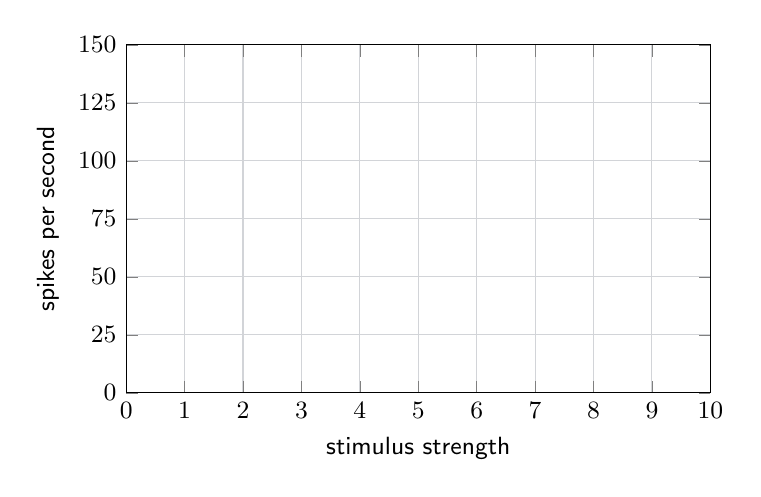
\begin{tikzpicture}
  \begin{axis}[width=9cm, height=6cm, xmin=0, xmax=10, ymin=0, ymax=150, xtick={0,1,...,10}, ytick={0,25,...,150},
      grid=both, grid style={kgrey!25}, xlabel={stimulus strength}, ylabel={spikes per second},
      tick label style={font=\small}, label style={font=\small}]
    \addplot[draw=none] coordinates {(0,0)};
  \end{axis}
\end{tikzpicture}
\end{minipage}

\medskip
\textbf{1.} Describe the pattern in one sentence. This is what Edgar Adrian found in 1926.
\lines{1}
\textbf{2.} Adrian also found \textbf{adaptation}: with a constant stimulus, the rate slowly falls. Give one everyday example of no longer noticing something that is still there.
\lines{1}

% ============================ PAGE 8 =================================
\newpage
\pagehead{Study cards}

\begin{studycard}[title={Edgar Adrian and the first single-neuron recordings (1926)}]
\textbf{Found:} with new valve amplifiers, Adrian recorded single sensory nerve fibres. He showed that their spikes are all or none, that the firing rate rises with stimulus strength (a heavier weight on a frog's muscle gave more spikes per second), and that the rate falls during a constant stimulus (adaptation). Nobel Prize, 1932, shared with Charles Sherrington \emph{(Rieke et al., 1997, Ch.~1)}.
\end{studycard}

\begin{studycard}[title={Hodgkin and Huxley: the spike in equations (1952)}]
\textbf{Found:} using the squid giant axon, they measured sodium and potassium currents separately and wrote equations for doors that open and close with voltage. The equations predicted a pulse with the shape and speed of a real spike. Nobel Prize, 1963. Spike Lab runs these equations.
\end{studycard}

\begin{studycard}[title={Neher and Sakmann: one door at a time (1976)}]
\textbf{Found:} with the patch-clamp method, they recorded the tiny current through a single channel protein as it flicked open and shut. Nobel Prize, 1991.
\end{studycard}

\begin{studycard}[title={Why spikes? (Hodgkin and Rushton, 1946)}]
\textbf{Found:} without active doors, a voltage change spreads and fades within about a millimetre. A spike is rebuilt along the axon, so it can travel a metre, from fingertip to spinal cord, at full size.
\end{studycard}

\begin{studycard}[title={Timing matters too (Mainen and Sejnowski, 1995)}]
\textbf{Found:} a cortical neuron given the same flickering input twice fires at nearly the same moments, to within about a millisecond. Spikes can carry information in \emph{when} they happen, not just how many.
\end{studycard}

\begin{studycard}[title={The homunculus (Rieke et al., 1997)}]
\textbf{Idea:} the brain receives only spike trains. A ``little person'' watching them explains nothing. Yet when scientists record spikes and ask what they mean, they take that little person's place: understanding the neural code means being able to read the spikes.
\end{studycard}

% ============================ PAGE 9 =================================
\newpage
\pagehead{Answers (check after class)}

\textbf{Part 1.} Threshold at strength \textbf{4.5} (at 4.0 the voltage only reaches about $-59$ mV). Peaks: about $+37$ mV at threshold, about $+41$ mV at strength 10. More than twice the push, nearly the same spike: \textbf{all or none}. Prediction: about the same.

\textbf{Part 2.} Sodium doors open first. Sodium blocker: \textbf{no spike}. Time above 0 mV: about \textbf{1.2 ms} normally, about \textbf{2.6 ms} with the potassium blocker. Up: \Na\ rushes in through voltage-gated doors. Down: \Na\ doors lock shut and \K\ flows out. Lidocaine blocks sodium doors in the nerves near the injection, so pain spikes cannot be made or passed on.

\textbf{Part 3.} Shortest gaps: \textbf{13 ms} at strength 8, \textbf{12 ms} at strength 10. (1) Relative. (2) About $1000 \div 1 = $ \textbf{1000 spikes per second} at most; most neurons fire far more slowly. (3) The patch just behind a travelling spike is still refractory, so the spike can only move forwards.

\textbf{Part 4.} About 5 (one spike only), 80, 90, 105 and 115 spikes per second for strengths 1, 3, 5, 7 and 10. (1) The stronger the stimulus, the more spikes per second: \textbf{rate coding}. The squid model jumps from one spike to about 65 per second; real sensory neurons can also fire slowly. (2) Examples: a watch on your wrist, clothes on your skin, the hum of a fan, a smell in a room after a while.

\textbf{Exit ticket.} (1) Past threshold a spike is full size; below it, there is no spike. (2) Sodium up, potassium down. (3) By firing more spikes per second (and sometimes by when spikes arrive).

% ============================ PAGE 10 ================================
\newpage
\pagehead{Sources}
\small
\begin{itemize}[leftmargin=1.2em,itemsep=2pt]
\item Adrian, E.\,D.\ (1926). The impulses produced by sensory nerve endings. Part 1. \emph{Journal of Physiology} 61, 49--72.
\item Adrian, E.\,D., \& Zotterman, Y.\ (1926). The impulses produced by sensory nerve-endings. Part 2: The response of a single end-organ. \emph{Journal of Physiology} 61, 151--171.
\item Bear, M.\,F., Connors, B.\,W., \& Paradiso, M.\,A.\ (2016). \emph{Neuroscience: Exploring the Brain} (4th ed.), Chapter 4.
\item de Leeuw, J.\,R.\ (2015). jsPsych: a JavaScript library for creating behavioral experiments in a web browser. \emph{Behavior Research Methods} 47, 1--12.
\item Hodgkin, A.\,L., \& Huxley, A.\,F.\ (1952). A quantitative description of membrane current and its application to conduction and excitation in nerve. \emph{Journal of Physiology} 117, 500--544.
\item Hodgkin, A.\,L., \& Rushton, W.\,A.\,H.\ (1946). The electrical constants of a crustacean nerve fibre. \emph{Proceedings of the Royal Society B} 133, 444--479.
\item Mainen, Z.\,F., \& Sejnowski, T.\,J.\ (1995). Reliability of spike timing in neocortical neurons. \emph{Science} 268, 1503--1506.
\item Neher, E., \& Sakmann, B.\ (1976). Single-channel currents recorded from membrane of denervated frog muscle fibres. \emph{Nature} 260, 799--802.
\item Rieke, F., Warland, D., de Ruyter van Steveninck, R., \& Bialek, W.\ (1997). \emph{Spikes: Exploring the Neural Code}. MIT Press. Chapter 1.
\item Spike Lab: the Hodgkin--Huxley (1952) model of the squid giant axon at 6.3\,\textdegree C. The ``potassium blocker'' removes 90\% of the voltage-opened potassium current and keeps the resting part.
\end{itemize}
\end{document}
